\documentclass[11pt,preprint, authoryear]{elsarticle}

\usepackage{lmodern}
%%%% My spacing
\usepackage{setspace}
\setstretch{1.2}
\DeclareMathSizes{12}{14}{10}{10}

% Wrap around which gives all figures included the [H] command, or places it "here". This can be tedious to code in Rmarkdown.
\usepackage{float}
\let\origfigure\figure
\let\endorigfigure\endfigure
\renewenvironment{figure}[1][2] {
    \expandafter\origfigure\expandafter[H]
} {
    \endorigfigure
}

\let\origtable\table
\let\endorigtable\endtable
\renewenvironment{table}[1][2] {
    \expandafter\origtable\expandafter[H]
} {
    \endorigtable
}


\usepackage{ifxetex,ifluatex}
\usepackage{fixltx2e} % provides \textsubscript
\ifnum 0\ifxetex 1\fi\ifluatex 1\fi=0 % if pdftex
  \usepackage[T1]{fontenc}
  \usepackage[utf8]{inputenc}
\else % if luatex or xelatex
  \ifxetex
    \usepackage{mathspec}
    \usepackage{xltxtra,xunicode}
  \else
    \usepackage{fontspec}
  \fi
  \defaultfontfeatures{Mapping=tex-text,Scale=MatchLowercase}
  \newcommand{\euro}{€}
\fi

\usepackage{amssymb, amsmath, amsthm, amsfonts}

\def\bibsection{\section*{References}} %%% Make "References" appear before bibliography

\usepackage{lineno}
\linenumbers

\usepackage[round]{natbib}
\bibliographystyle{plainnat}

\usepackage{longtable}
\usepackage[margin=defaultcm,bottom=2cm,top=2.5cm, includefoot]{geometry}
\usepackage{fancyhdr}
\usepackage[bottom, hang, flushmargin]{footmisc}
\usepackage{graphicx}
\numberwithin{equation}{section}
\numberwithin{figure}{section}
\numberwithin{table}{section}
\setlength{\parindent}{0cm}
\setlength{\parskip}{1.3ex plus 0.5ex minus 0.3ex}
\usepackage{textcomp}
\renewcommand{\headrulewidth}{0.2pt}
\renewcommand{\footrulewidth}{0.3pt}

\usepackage{array}
\newcolumntype{x}[1]{>{\centering\arraybackslash\hspace{0pt}}p{#1}}

%%%%  Remove the "preprint submitted to" part. Don't worry about this either, it just looks better without it:
\makeatletter
\def\ps@pprintTitle{%
  \let\@oddhead\@empty
  \let\@evenhead\@empty
  \let\@oddfoot\@empty
  \let\@evenfoot\@oddfoot
}
\makeatother

 \def\tightlist{} % This allows for subbullets!

\usepackage{hyperref}
\hypersetup{breaklinks=true,
            bookmarks=true,
            colorlinks=true,
            citecolor=blue,
            urlcolor=blue,
            linkcolor=blue,
            pdfborder={0 0 0}}


% The following packages allow huxtable to work:
\usepackage{siunitx}
\usepackage{multirow}
\usepackage{hhline}
\usepackage{calc}
\usepackage{tabularx}
\usepackage{booktabs}
\usepackage{caption}


\urlstyle{same}  % don't use monospace font for urls
\setlength{\parindent}{0pt}
\setlength{\parskip}{6pt plus 2pt minus 1pt}
\setlength{\emergencystretch}{3em}  % prevent overfull lines
\setcounter{secnumdepth}{5}

%%% Use protect on footnotes to avoid problems with footnotes in titles
\let\rmarkdownfootnote\footnote%
\def\footnote{\protect\rmarkdownfootnote}
\IfFileExists{upquote.sty}{\usepackage{upquote}}{}

%%% Include extra packages specified by user

%%% Hard setting column skips for reports - this ensures greater consistency and control over the length settings in the document.
%% page layout
%% paragraphs
\setlength{\baselineskip}{12pt plus 0pt minus 0pt}
\setlength{\parskip}{12pt plus 0pt minus 0pt}
\setlength{\parindent}{0pt plus 0pt minus 0pt}
%% floats
\setlength{\floatsep}{12pt plus 0 pt minus 0pt}
\setlength{\textfloatsep}{20pt plus 0pt minus 0pt}
\setlength{\intextsep}{14pt plus 0pt minus 0pt}
\setlength{\dbltextfloatsep}{20pt plus 0pt minus 0pt}
\setlength{\dblfloatsep}{14pt plus 0pt minus 0pt}
%% maths
\setlength{\abovedisplayskip}{12pt plus 0pt minus 0pt}
\setlength{\belowdisplayskip}{12pt plus 0pt minus 0pt}
%% lists
\setlength{\topsep}{10pt plus 0pt minus 0pt}
\setlength{\partopsep}{3pt plus 0pt minus 0pt}
\setlength{\itemsep}{5pt plus 0pt minus 0pt}
\setlength{\labelsep}{8mm plus 0mm minus 0mm}
\setlength{\parsep}{\the\parskip}
\setlength{\listparindent}{\the\parindent}
%% verbatim
\setlength{\fboxsep}{5pt plus 0pt minus 0pt}



\begin{document}

\begin{frontmatter}  %

\title{A multivariate GARCH Model of real estate and investment trusts:
Evidence from South Africa and global markets}

% Set to FALSE if wanting to remove title (for submission)




\author[Add1]{Lintle Balone}
\ead{lintlebalone25@gmail.com}





\address[Add1]{Department of Economics, Stellenbosch University, Cape Town, South
Africa}


\begin{abstract}
\small{
Using the high frequency data for five periods we examine the
correlations between South African REITs and selected global countries.
We study the various Reits companies of the Morgan Stanly Capital
International (MSCI). Our analysis shows that South African reits are
the least volatile stocks in relation to other stocks. Finally, there is
strong evidence that South African reits and global reits have a low
correlation, possibly increasing th benefits to portfolio
diversification when the market is highly volatile. This is a very
signifcant result and has not been explored in depth so far in South
African context. These results will be useful in model building for
prediction of price movement and portfolio management.
}
\end{abstract}

\vspace{1cm}

\begin{keyword}
\footnotesize{
Multivariate GARCH \\ \vspace{0.3cm}
\textit{JEL classification} L250 \sep L100
}
\end{keyword}
\vspace{0.5cm}
\end{frontmatter}



%________________________
% Header and Footers
%%%%%%%%%%%%%%%%%%%%%%%%%%%%%%%%%
\pagestyle{fancy}
\chead{}
\rhead{}
\lfoot{}
\rfoot{\footnotesize Page \thepage\textbackslash{}}
\lhead{}
%\rfoot{\footnotesize Page \thepage\ } % "e.g. Page 2"
\cfoot{}

%\setlength\headheight{30pt}
%%%%%%%%%%%%%%%%%%%%%%%%%%%%%%%%%
%________________________

\headsep 35pt % So that header does not go over title




\hypertarget{introduction}{%
\section{\texorpdfstring{Introduction
\label{Introduction}}{Introduction }}\label{introduction}}

Recently, the linkage between real estate investment and trusts (REITs)
and finance has been a crucial field of interest, due to the increasing
importance of property as a significant asset class in investment. This
has been further enhanced by the economic condition of the United States
relating to the systematic defaulting of subprime borrowers.
Consequently, this has influenced how investors diversify their
portfolios. Portfolio diversification means holding equities across
various sectors (Stephens and Tiddens
\protect\hyperlink{ref-stephensinter2017}{2017}). However; this paper
will specifically analyses REITs returns between different countries.
Real estate investment and trusts (REITs) returns have been
significantly examined in the literature, however; reviews that have
examined the REITs return comovements between South Africa and different
countries are have not been explored in greater depth. Relatively,
little research has been performed in the South African REITs compared
to other REITs markets (Nurick et al.
\protect\hyperlink{ref-nurick2018investigation}{2018}; Anderson
\protect\hyperlink{ref-anderson2016place}{2016}).

The purpose of this paper is to analyze the co-movements and the
portfolio diversification of the South African REITs and its trading
partners. Furthermore, the Multivariate (MV) GARCH modelling is used to
examine the conditional correlations between REITs in different
countries. The rationale for multivariate (MV) GARCH modelling technique
is for investors to include time-varying correlations in their portfolio
selection, hence this paper explores their properties. The results offer
valuable insights into which the South African REITs appear to provide
better diversification. Secondly, the volatility plot indicates that
South Africa has very low volatility compared to Indonesia, Thailand and
Israel reits.

The paper is structured as follows: Section \ref{Literature Review}
presents the relevant literature. Section \ref{Data} discusses the data
used in the paper and section \ref{Methodology} provides a comprehensive
methodology employed in this paper. Section \ref{Results} presents the
results of the estimated models. Section \ref{Conclusion} concludes.
Lastly, section \ref{Appendix} presents the appendix.

\hypertarget{literature-review}{%
\section{\texorpdfstring{Literature Review
\label{Literature Review}}{Literature Review }}\label{literature-review}}

The literature significant to this study focuses on South African and
international Reits in the light of portfolio management. The driving
factors cited in the literature for international investment are
diversification and risk-adjusted-performance (Worzala
\protect\hyperlink{ref-worzala1994overseas}{1994}; Austin and Geurts
\protect\hyperlink{ref-austin1995risk}{1995}; Worzala and Sirmans
\protect\hyperlink{ref-worzala2003investing}{2003}). This trade-off
between risk and return is based on a conventional portfolio theory that
prudent investors choose portfolios with the lowest risk for a specific
level of return. In other words, diversification of portfolios creates
incentives for risk reduction, such as diversification of real estate
portfolios to include offshore investments without reducing returns
(Austin and Geurts \protect\hyperlink{ref-austin1995risk}{1995}). It is
also worth noting that, in portfolio theory, low correlations between
dissimilar stocks will increase diversification potential and decrease
portfolio risk (Stephens and Tiddens
\protect\hyperlink{ref-stephensinter2017}{2017}). Put differently, the
various types of investments should not follow the same pattern in the
market. Therefore, the rewards of portfolio diversification weigh
heavily on the correlation framework of the stock markets examined.

Bruin et al. (\protect\hyperlink{ref-bruin2009real}{2009}) stated that
in real estate investment, portfolio diversification benefits can be
accomplished by diversifying across property types and geographical
regions. It has been found that various forms of international real
estate have weak correlations with other types of investment, hence
contribute to a well-diversified portfolio. Moreover, the literature has
well-documented evidence that there is a weak correlation between
emerging markets and developed markets resulting in diversification
benefits (Basu and Gupta \protect\hyperlink{ref-basu2005benefits}{2005};
Barry, Peavy Jr, and Rodriguez
\protect\hyperlink{ref-barry1998performance}{1998}; Magas
\protect\hyperlink{ref-magas2007changing}{2007}). However; the
perception that there is a weak correlation between emerging markets and
developed markets is deteriorating. For instance, Wong et al.
(\protect\hyperlink{ref-wong2004relationship}{2004}) examined the
co-movement between stock markets in Asian emerging markets and
developed countries using cointegration analysis. They found that there
is an increasing correlation between most emerging and developed
markets. Chancharat and Valadkhani
(\protect\hyperlink{ref-chancharat2007empirical}{2007}) employed
cointegration and causality tests between major international stock
markets and Thailand and found a high correlation between Thailand and
other international markets.

The results of various studies on diversification of real estate are
based on modern portfolio theory (MPT) (Paul, Robert, and Carl
\protect\hyperlink{ref-paul1991risk}{1991}; Seiler, Webb, and Myer
\protect\hyperlink{ref-seiler1999diversification}{1999}; Wilson and
Zurbruegg \protect\hyperlink{ref-wilson2003international}{2003}).
However; Theron and Van Vuuren
(\protect\hyperlink{ref-theron2018maximum}{2018}) stated that the Modern
portfolio approach is rather flawed because it assumes all parameters
are known accurately. These parameters (covariances, variances and
expected returns) are estimated not necessarily known with certainty. As
a result, this uncertainty in parameters leads to estimation risk, which
in turn also leads to suboptimal investor financial choices. Modern
portfolio theorem was also criticized for the inefficient performance of
many institutional portfolios during the financial crisis of 2008/2009
because most portfolios were focused on Markowitz's optimization of
portfolios, a mechanism that was widely assumed would provide the
necessary diversification to prevent seriously negative portfolios
(Choueifaty, Froidure, and Reynier
\protect\hyperlink{ref-choueifaty2013properties}{2013}). Modern
portfolio models also introduced assets with weak equity correlations,
but most asset class correlations increased during the crisis and
expected diversification benefits were negligible. Therefore, there is a
need for alternative investment ideas.

In addition to these studies, some focus primarily on developed markets
in the US, Canada, Europe and Japan, for instance (Bond and Glascock
\protect\hyperlink{ref-bond2006performance}{2006}; Basse, Friedrich, and
Bea \protect\hyperlink{ref-basse2009reits}{2009}; Moss and Prima
\protect\hyperlink{ref-moss2014asia}{2014}). Bond and Glascock
(\protect\hyperlink{ref-bond2006performance}{2006}) found that real
estate has contributed substantially to the overall portfolio outcomes
in terms of higher returns and decreases risk. Secondly, the authors are
consistent with other researchers that real estate investment performs
well during periods of market change. Basse, Friedrich, and Bea
(\protect\hyperlink{ref-basse2009reits}{2009}) found that investing in
US REITs was riskier compared to investment in utility stocks. Further
analysis linked this result to the economic state and financial crisis
in the US. Moss and Prima (\protect\hyperlink{ref-moss2014asia}{2014})
examined the correlation between developed Asian REITs and other
developed countries and found that there are interdependent linkages
among the REITs market of developed countries.

Certain literature studies analyze stock price linkages between emerging
stock markets only, without capturing major stock influences in
developed countries (Sharma and Wongbangpo
\protect\hyperlink{ref-sharma2002long}{2002}; San Ong et al.
\protect\hyperlink{ref-san2012malaysian}{2012}; Yang, Kolari, and Min
\protect\hyperlink{ref-yang2003stock}{2003}). Their findings suggest
that Reits provided a better diversification post-financial crisis.
Sharma and Wongbangpo (\protect\hyperlink{ref-sharma2002long}{2002}) and
Yang, Kolari, and Min (\protect\hyperlink{ref-yang2003stock}{2003})
found low evidence of the correlation among Asian stock markets. Also,
some studies analyses the interrelationships between developed and
emerging markets. For instance, Pham
(\protect\hyperlink{ref-pham2012dynamics}{2012}) examined the dynamics
of returns and volatility in emerging and developed markets and found
that correlations among emerging Reits are lower than those among
developed countries.

In investment of real estate, the advantages of portfolio
diversification can be accomplished by introducing international real
estate into the portfolio. Worzala and Sirmans
(\protect\hyperlink{ref-worzala2003investing}{2003}) found that with the
introduction of international real estate to the portfolio, portfolio
performance improves significantly. Worzala and Sirmans
(\protect\hyperlink{ref-worzala2003investing}{2003}) discovered that
investment in securities linked to international real estate offers
additional diversification advantages. Similarly, Niskanen and
Falkenbach (\protect\hyperlink{ref-niskanen2010reits}{2010}) claimed
that international diversification of REITs investment is suggested to
reduce exposure due to economic uncertainties within countries.
Nonetheless, the question asked in this research is ``are there any
types of interdependence or dynamic correlation between South Africa and
international markets?

\hypertarget{data}{%
\section{\texorpdfstring{Data \label{Data}}{Data }}\label{data}}

The aim of this study is to investigate the correlation of the Reits
market of South Africa and its trading partner countries to access the
diversification benefits. The return series are time-varying, intradays
as well as over days. In the light of this, it is undesirable to apply
models assuming time-invariant conditional variances.

We picked a sample of 10 best performing stocks and 10 worst performing
stocks,includsive of South Africa. This selection was made because an
investor can reduce the overall risk of his or her portfolio by owning
multiple Reits which perform differently. All data is obtained from
Morgan Stanely Capital International (MSCI) and encompasses of high
frequency data of different time frames.

The stock value indexes are expressed in US dollars to avoid exchange
rates fluctuations. For further analysis, the continuously compounded
daily returns are calculated by taking the log difference of each listed
company as follows:

\begin{align} 
r_{ki,t} = \ln (\frac{P_{k,t}}{P_{k,t-7}})
\label{eq1} \\ \notag 
\end{align}

Table \ref{tab1} shows all the tickers that have been used in this
analysis. In Table \ref{tab2} it is reported that, daily mean returns
were highest for the MXEU0RE index and lowest for the MXZA0RL with
values of 9.872380 and -9.023962. During the period, daily returns for
most indices are negatively skewed. The MMXWD0RE was the most negatively
skewed with a skewness value of -0.611994373 indicating an extreme left
tale. In addition to this, MXTHORL was the most positively skewed.
Similarly, the daily returns for all indices exhibit excess positive
kurtosis with MXMY0RL having the highest kurtosis. This is the distinct
characteristic of financial data and suggests that the series is not
normally distributed.

According to the normality test both daily returns and absolute returns
are non normal for all indices. The null hypothesis of normality test
was rejected for all indices..\footnote{We tested for normality using
  the Jarque-Bera normality test and the results indicate that the
  returns are not normally distributed.} In Figure \ref{Figure3} we note
that the return series appears to be nearly stable with an average
return of approximately zero, however the variability of the data
changes over time.

\hypertarget{methodology}{%
\section{Methodology}\label{methodology}}

The empirical analysis is undertaken using an MGARCH framework
considering a stochastic process \(y_t\), of a continuously compounded
daily returns. The first step in this analysis is to obtain the GARCH
estimates for the univirate volatility estimates fo each series. The
study employs the GARCH(1,1) univariate specification. The standard
GARCH(1,1) specification model is written in equation \ref{eq1} as
follows:

\begin{align}  
y_t = \mu_t + \varepsilon_t \label{eq1} \\ \notag 
    varepsilon_t = \sigma_t.z_t \\ \notag 
  sigma_t^{2} = \alpha + \beta_1 e_{t-1}^2 + \beta_1          sigma_{t-1}^2 \\ \notag
z_t \sim  N(0,I) \notag
\end{align}

The paper also employs the parsimonious DCC MV GARCH modelling
techniques of {[}engle2002dynamic{]}. The DCC model provides an easy and
parsimonious way of modeling multivariate volatility. The DCC model can
be described as follows:

\begin{equation} \label{eq2}
H_t = D_t.R_t.D_t.\\ \notag
\end{equation}

The equation \ref{eq2} splits the variance covariance matrix into
identical diagonal matrices and an estimate of time varying correlation.
\(R_t\) refers to time varying conditional correlations.

The diagonal matrices are defined as:

\begin {equation} \label {eq3}
D_t = diag(h_t^{1/2}, h_t^{1/2}).
 \end{equation}

Then we define the dynamic conditional correlation structure. This is
shown in \ref{eq4} below:

\begin{align}  \label{eq4}
Q_{ij,t} &= \bar Q + a\left(z_{t - 1}z'_{t - 1} - \bar{Q} \right) + b\left( Q_{ij, t - 1} - \bar{Q} \right) \hfill \\ \notag  &= (1 - a - b)\bar{Q} + az_{t - 1}z'_{t - 1} + b.Q_{ij, t - 1} \notag
\end{align}

\(Q_{ij,t}\) is the unconditional variance between series i and j.
\(\bar{Q}\) is the unconditional covarience between univariate series
estimated in step 1. The non-negative parameters are represented by a
and b and they must satisfy a + b \textless{} 1.

Equation \ref{eq4} is employed in order to estimate \(R_t\) as:

\begin{align}\label{eq5}
R_t &= diag(Q_t)^{-1/2}Q_t.diag(Q_t)^{-1/2}. 
\end{align}

Equation \ref{eq5} has bivariate elements that can be shown in the
equation below.

\begin{align} \label{eq6}
R_t &= \rho_{ij,t} = \frac{q_{i,j,t}}{\sqrt{q_{ii,t}.q_{jj,t}}} 
\end{align}

Writing out a complete DCC model is then constructed as shown in
\ref{eq7} below:

\begin{align} \label{eq7}
\varepsilon_t &\thicksim  N(0,D_t.R_t.D_t) \notag \\
D_t^2 &\thicksim \text{Univariate GARCH(1,1) processes $\forall$ (i,j), i $\ne$ j} \notag \\
z_t&=D_t^{-1}.\varepsilon_t \notag \\
R_t &= Diag(Q_t^{-1}).Q_t.Diag({Q_t}^{-1}) \notag \\
{Q}(1-a-b)+a(z_t'z_t)+b(Q_{t-1}) \notag \\
\end{align}

\hypertarget{results}{%
\section{\texorpdfstring{Results
\label{Results}}{Results }}\label{results}}

Section \ref{Standard Univariate GARCH(1,1) Model} discusses results of
the standard univariate GARCH(1,1) model. Section \ref{The DCC Model}
presents the results of the DCC model.

\hypertarget{standard-univariate-garch11-model}{%
\subsection{\texorpdfstring{Standard Univariate GARCH(1,1) Model
\label{Standard Univariate GARCH(1,1) Model}}{Standard Univariate GARCH(1,1) Model }}\label{standard-univariate-garch11-model}}

The graph below report Reits conditional volatility of the respective
GARCH model. Volatility is the degree to which the trade price series
varies over time. Even though volatility patterns look almost similar
for all indices, differences between the volatility levels of indices
can be seen. It is is evident from the graph that other stocks are
highly volatile throughout the periods. Indonesia, Thailand and Israel
real estate are amongst the higly volatile stocks. Indonesia real estate
display the highest spikes upward compared to other reits in other
periods such as . This is unsurprising because these are emerging
coutries where returns are classified to be higly volatile in such
regions. The graph also shows that South African reit index is the least
volatily, therefore it results in lower expected losses.

The findings in Table \ref{tab1} also show the volatality output of the
reits indices measured by the standard deviation. Indonesia reits
display the highest volatility amongst all the indices, however with one
of the lowest daily returns. The MXWD0RE reits exhibits the lowest
volatility amongst all the indiced. Moreover, it is apparent that one of
the least volatile indices is the South Afican reit index which can
offer valuable insights into diversification potential. Summing up,
higher average returns are connected with larger risk exposure in
Chinese real estate which coincides with the traditional asset pricing
theory.

\begin{figure}[H]

{\centering 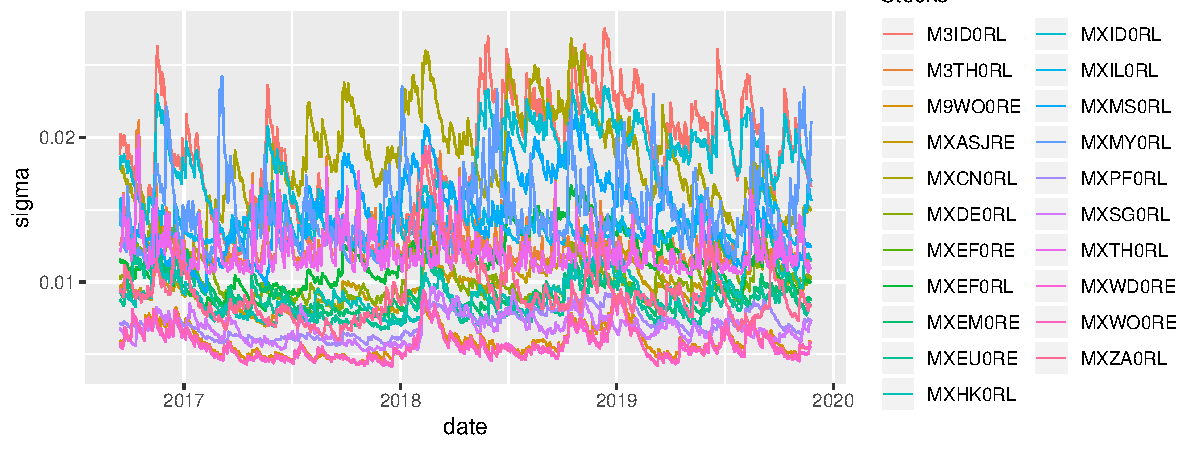
\includegraphics{Template_files/figure-latex/vol.datplotReits-1} 

}

\caption{Volatility of each asset \label{Figure1}}\label{fig:vol.datplotReits}
\end{figure}

The next step is to fit our DCC model utilizing the residuals that we
have obtained when fitting the GARCH model. The dynamic conditional
correlations are shown in figure \ref{Figure2} below:

\hypertarget{the-dcc-model}{%
\subsection{\texorpdfstring{The DCC Model
\label{The DCC Model}}{The DCC Model }}\label{the-dcc-model}}

The time-varying correlation offers an insight into the underlying
comovement structures of a portfolio (Katzke
\protect\hyperlink{ref-katzke2019multivariate}{2019}). Basically the
DCC-GARCH model estimates conditional volatilities and correlations in
two steps ({\textbf{???}}). It should be noted that the comovements
between stocks is fundamental to investors and investment managers, as
it provides valuable insights into proper diversification. If there is a
high correlation between two stocks, then an investor is faced with low
diversification.

Firstly, we clean the daily returns by using the Boundt's technique.
This is extremely crucial because it cleans outliers from the return
data. Subsequently, we run the MV heteroskedasticity tests. The MARCH
test indicates that all the MV portmanteau tests reject the null of no
conditional heteroskedasticity, motivating our use of MVGARCH models.

\begin{verbatim}
## Estimates:  0.95 0.02465337 11.48087 
## st.errors:  0.004974356 0.001442199 0.7267799 
## t-values:   190.9795 17.09429 15.7969
\end{verbatim}

\begin{figure}[H]

{\centering 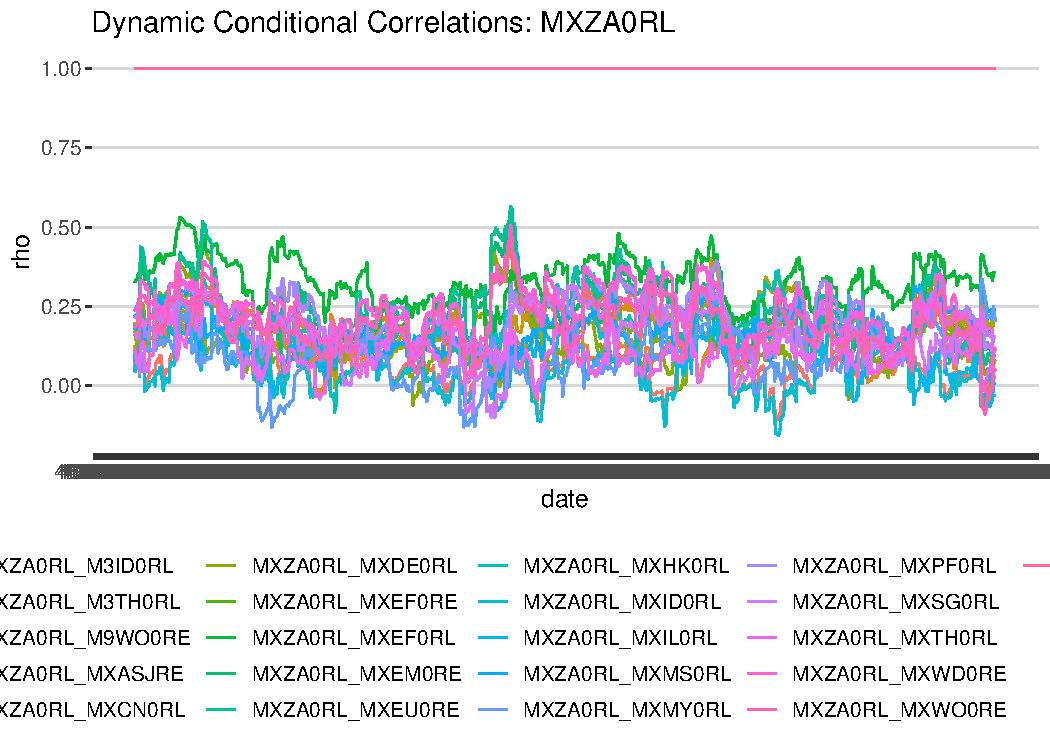
\includegraphics{Template_files/figure-latex/DCC.plot-1} 

}

\caption{Dynamic Conditional Correlations for Each Asset Relative to the SA Reits \label{Figure2}}\label{fig:DCC.plot}
\end{figure}

In terms of the interpretation, the lower the dynamic correlations, the
higher the diversification. This is because low correlation reduces the
volatility of the portfolioas a whole. The results in \ref{Figure2}
confirm that the conditional correlations of South Africa and global
reits returns are highly dynamic and time varying. Moreover, it seems
that the volatilities of SA reits and global reits comove together. From
Figure \ref{Figure2} it is apparent that the correlations between
MXZA0RL\_MXEU0RE and MXZA0RL\_MXEM0RE are relatively low. These results
are consistent with Basu and Gupta
(\protect\hyperlink{ref-basu2005benefits}{2005}); Barry, Peavy Jr, and
Rodriguez (\protect\hyperlink{ref-barry1998performance}{1998}); Magas
(\protect\hyperlink{ref-magas2007changing}{2007}) results that there is
a weak correlation between emerging markets and developed markets
resulting in diversification benefits. It is also evident that the
correlation between MXZA0RL\_M9WO0RE AND MXZA0RL\_MXWO0RE reits is
relatively high.

It is worth noting that the dynamic correlations make it clear that the
diversifaction opportunities of the included REITS are not entirely
constant over time. In conclusion, the results in figure \ref{Figure2}
confirm that the conditional correlations of South African reits and
global reits are dynamic and time varying.

\hypertarget{conclusion}{%
\section{\texorpdfstring{Conclusion
\label{conclusion}}{Conclusion }}\label{conclusion}}

In this study we address one of the most important questions concerning
conventional and morden portfolio management, i.e., the dynanmic
conditional correlation between South African reits and global reits.
Correlation of reits plays a fundamental role in asset allocation risk
management and portfolio managed. Despite its significance this
phenomena has been significantly neglected in ermeging markets
regardless of their high returns and attractive potential for
diversification. We have carried out an analysis of the Multivariate
modelling for a period of five years. This time frame contains periods
of small and large fluctuations and therefore provides a good example
for understanding and examining the reits market behaviour. As expected,
the financial data is not normally distributed and exhibit excess
kurtios and skeweness.

The empirical results support the assumption of dynamic conditional
correlations and there was evident evidence of time varying correlations
between South Africa and global reits. Moreover, these correlation are
very low, therefore, we believe our results can offer a comprehensive
understanding of the dynamic correlations between South African reits
and global reits in an emerging market setting which is valuable for
financial researchers, international investors, investment managers and
risk analysts. In a nutshell, South Africa can offer diversification
opportunities to investors during high periods of volatility when stocks
are extremely risky. Therefore, investors should invest in stocks that
do not comove such as South Africa.

\hypertarget{appendix}{%
\section{Appendix}\label{appendix}}

\begin{table}[H]
\centering
\begin{tabular}{rll}
  \hline
 & Ticker & Description \\ 
  \hline
1 & M3TH0RL & Thailand \\ 
  2 & MXCN0RL & China \\ 
  3 & MXDE0RL & Germany \\ 
  4 & MXEF0RL & EM Real Estate \\ 
  5 & MXHK0RL & Hong Kong \\ 
  6 & MXIL0RL & Israel \\ 
  7 & MXMS0RL & EM Asia \\ 
  8 & MXPF0RL & AC Pacific \\ 
  9 & MXSG0RL & Singapore \\ 
  10 & MXTH0RL & Thailand \\ 
  11 & M3ID0RL & Indonesia \\ 
  12 & M9WO0RE & World \\ 
  13 & MXASJRE & AC Asia ex Japan \\ 
  14 & MXEF0RE & EM Real Estate \\ 
  15 & MXEM0RE & EMU Real Estate \\ 
  16 & MXEU0RE & Europe \\ 
  17 & MXID0RL & Indonesia \\ 
  18 & MXMY0RL & Malaysia \\ 
  19 & MXWD0RE & ACWI Index \\ 
  20 & MXWO0RE & World \\ 
  21 & MXZA0RL & South Africa \\ 
   \hline
\end{tabular}
\caption{Asset description Table \label{tab1}} 
\end{table}

\begin{table}[H]
\centering
\begin{tabular}{rlrrrrrrrrrr}
  \hline
 & group1 & vars & mean & sd & median & trimmed & min & max & skew & kurtosis & se \\ 
  \hline
X11 & M3ID0RL & 1.00 & -0.00 & 0.02 & 0.00 & -0.00 & -0.08 & 0.08 & 0.20 & 1.53 & 0.00 \\ 
  X12 & M3TH0RL & 1.00 & 0.00 & 0.01 & 0.00 & 0.00 & -0.06 & 0.08 & 0.31 & 2.54 & 0.00 \\ 
  X13 & M9WO0RE & 1.00 & 0.00 & 0.01 & 0.00 & 0.00 & -0.03 & 0.02 & -0.54 & 1.37 & 0.00 \\ 
  X14 & MXASJRE & 1.00 & 0.00 & 0.01 & 0.00 & 0.00 & -0.04 & 0.05 & -0.20 & 1.90 & 0.00 \\ 
  X15 & MXCN0RL & 1.00 & 0.00 & 0.02 & 0.00 & 0.00 & -0.08 & 0.07 & 0.01 & 1.61 & 0.00 \\ 
  X16 & MXDE0RL & 1.00 & 0.00 & 0.01 & 0.00 & 0.00 & -0.06 & 0.06 & -0.29 & 3.29 & 0.00 \\ 
  X17 & MXEF0RE & 1.00 & 0.00 & 0.01 & 0.00 & 0.00 & -0.05 & 0.05 & -0.17 & 1.47 & 0.00 \\ 
  X18 & MXEF0RL & 1.00 & 0.00 & 0.01 & 0.00 & 0.00 & -0.05 & 0.05 & -0.17 & 1.47 & 0.00 \\ 
  X19 & MXEM0RE & 1.00 & 0.00 & 0.01 & 0.00 & 0.00 & -0.05 & 0.03 & -0.33 & 1.42 & 0.00 \\ 
  X110 & MXEU0RE & 1.00 & 0.00 & 0.01 & 0.00 & 0.00 & -0.04 & 0.03 & -0.25 & 0.93 & 0.00 \\ 
  X111 & MXHK0RL & 1.00 & 0.00 & 0.01 & 0.00 & 0.00 & -0.06 & 0.08 & 0.25 & 6.21 & 0.00 \\ 
  X112 & MXID0RL & 1.00 & -0.00 & 0.02 & 0.00 & -0.00 & -0.06 & 0.07 & 0.27 & 1.36 & 0.00 \\ 
  X113 & MXIL0RL & 1.00 & 0.00 & 0.01 & 0.00 & 0.00 & -0.05 & 0.05 & 0.07 & 1.17 & 0.00 \\ 
  X114 & MXMS0RL & 1.00 & 0.00 & 0.02 & 0.00 & 0.00 & -0.07 & 0.06 & -0.06 & 1.45 & 0.00 \\ 
  X115 & MXMY0RL & 1.00 & -0.00 & 0.02 & 0.00 & -0.00 & -0.14 & 0.14 & -0.12 & 11.95 & 0.00 \\ 
  X116 & MXPF0RL & 1.00 & 0.00 & 0.01 & 0.00 & 0.00 & -0.04 & 0.03 & -0.47 & 1.74 & 0.00 \\ 
  X117 & MXSG0RL & 1.00 & 0.00 & 0.01 & 0.00 & 0.00 & -0.04 & 0.04 & -0.11 & 3.47 & 0.00 \\ 
  X118 & MXTH0RL & 1.00 & 0.00 & 0.01 & 0.00 & -0.00 & -0.05 & 0.07 & 0.40 & 2.21 & 0.00 \\ 
  X119 & MXWD0RE & 1.00 & 0.00 & 0.01 & 0.00 & 0.00 & -0.03 & 0.02 & -0.61 & 1.70 & 0.00 \\ 
  X120 & MXWO0RE & 1.00 & 0.00 & 0.01 & 0.00 & 0.00 & -0.02 & 0.02 & -0.57 & 1.55 & 0.00 \\ 
  X121 & MXZA0RL & 1.00 & -0.00 & 0.01 & 0.00 & -0.00 & -0.06 & 0.09 & 0.16 & 8.92 & 0.00 \\ 
   \hline
\end{tabular}
\caption{Descriptive Statistics Table \label{tab2}} 
\end{table}

\begin{figure}[H]

{\centering \includegraphics{Template_files/figure-latex/figure3-1} 

}

\caption{Daily log Reits Returns \label{Figure3}}\label{fig:figure3}
\end{figure}

\hypertarget{references}{%
\section*{References}\label{references}}
\addcontentsline{toc}{section}{References}

\hypertarget{refs}{}
\leavevmode\hypertarget{ref-anderson2016place}{}%
Anderson, Lloyd. 2016. ``A Place for Residential Reits in the South
African Reit Market.'' PhD thesis, University of Pretoria.

\leavevmode\hypertarget{ref-austin1995risk}{}%
Austin, Jaffe, and Tom G. Geurts. 1995. ``Risk and Real Estate
Investment: An International Perspective.'' \emph{Journal of Real Estate
Research} 11 (2): 117--30.

\leavevmode\hypertarget{ref-barry1998performance}{}%
Barry, Christopher B, John W Peavy Jr, and Mauricio Rodriguez. 1998.
``Performance Characteristics of Emerging Capital Markets.''
\emph{Financial Analysts Journal} 54 (1): 72--80.

\leavevmode\hypertarget{ref-basse2009reits}{}%
Basse, Tobias, Meik Friedrich, and E Vazquez Bea. 2009. ``REITs and the
Financial Crisis: Empirical Evidence from the Us.'' \emph{International
Journal of Business and Management} 4 (11): 3--10.

\leavevmode\hypertarget{ref-basu2005benefits}{}%
Basu, P, and R Gupta. 2005. ``Benefits of Diversification into Emerging
Equity Markets with Changing Correlations: An Australian Perspective.''
In \emph{18th Australian Finance and Banking Conference}, 14--16.

\leavevmode\hypertarget{ref-bond2006performance}{}%
Bond, Shaun A, and John L Glascock. 2006. ``The Performance and
Diversification Benefits of European Public Real Estate Securities.''
\emph{Available at SSRN 896524}.

\leavevmode\hypertarget{ref-bruin2009real}{}%
Bruin, Thomas, Rebecca Porterfield, Edward Graham, and Joseph Farinella.
2009. ``Real Estate Investment Trusts and Market Sentiment in the United
States \& Europe.'' \emph{Annals of the International Masters of
Business Administration at UNC Wilmington} 2 (1).

\leavevmode\hypertarget{ref-chancharat2007empirical}{}%
Chancharat, Surachai, and Abbas Valadkhani. 2007. ``An Empirical
Analysis of the Thai and Major International Stock Markets.''

\leavevmode\hypertarget{ref-choueifaty2013properties}{}%
Choueifaty, Yves, Tristan Froidure, and Julien Reynier. 2013.
``Properties of the Most Diversified Portfolio.'' \emph{Journal of
Investment Strategies} 2 (2): 49--70.

\leavevmode\hypertarget{ref-katzke2019multivariate}{}%
Katzke, N. F. 2019. ``Financial Econometrics Course: Multivariate
Volatility Modeling.''
\url{https://www.fmx.nfkatzke.com/posts/2019-09-06-practical-multivariate-volatility-modeling/}.

\leavevmode\hypertarget{ref-magas2007changing}{}%
Magas, I. 2007. ``The Changing Benefits of Global Equity Investing:
Developed and Emerging Markets, 1997--2007.'' \emph{Acta Oeconomica} 57
(4): 343--62.

\leavevmode\hypertarget{ref-moss2014asia}{}%
Moss, Alex, and AD Prima. 2014. ``Asia Pacific Listed Real Estate: A
Contextual Performance Analysis.''

\leavevmode\hypertarget{ref-niskanen2010reits}{}%
Niskanen, Jaakko, and Heidi Falkenbach. 2010. ``REITs and Correlations
with Other Asset Classes: A European Perspective.'' \emph{Journal of
Real Estate Portfolio Management} 16 (3): 227--39.

\leavevmode\hypertarget{ref-nurick2018investigation}{}%
Nurick, Saul, Luke Boyle, Greg Morris, Jacques Potgieter, and Oliver
Allen. 2018. ``An Investigation into the Relatively Low Uptake of
Residential Stock Within South African Real Estate Investment Trusts.''
\emph{Journal of African Real Estate Research} 3 (1): 61--80.

\leavevmode\hypertarget{ref-paul1991risk}{}%
Paul, Asabere, Kleiman Robert, and McGowan Carl. 1991. ``The Risk-Return
Attributes of International Real Estate Equities.'' \emph{Journal of
Real Estate Research} 6 (2): 143--51.

\leavevmode\hypertarget{ref-pham2012dynamics}{}%
Pham, Anh Khoi. 2012. ``The Dynamics of Returns and Volatility in the
Emerging and Developed Asian Reit Markets.'' \emph{Journal of Real
Estate Literature} 20 (1): 79--96.

\leavevmode\hypertarget{ref-san2012malaysian}{}%
San Ong, Tze, Boon Heng Teh, Chin Hooi Soh, and Yat Liang Yan. 2012.
``Malaysian Real Estate Investment Trusts: A Performance and Comparative
Analysis.'' \emph{International Journal of Economics and Finance} 4 (5):
p73.

\leavevmode\hypertarget{ref-seiler1999diversification}{}%
Seiler, Michael, James Webb, and Neil Myer. 1999. ``Diversification
Issues in Real Estate Investment.'' \emph{Journal of Real Estate
Literature} 7 (2): 163--79.

\leavevmode\hypertarget{ref-sharma2002long}{}%
Sharma, Subhash C, and Praphan Wongbangpo. 2002. ``Long-Term Trends and
Cycles in Asean Stock Markets.'' \emph{Review of Financial Economics} 11
(4): 299--315.

\leavevmode\hypertarget{ref-stephensinter2017}{}%
Stephens, David, and Charlotte van Tiddens. 2017. ``Inter-Sector Return
Correlations Between South Africa, the United States, the United Kingdom
and Europe: Evidence from the Dcc Multivariate Garch Model.''

\leavevmode\hypertarget{ref-theron2018maximum}{}%
Theron, Ludan, and Gary Van Vuuren. 2018. ``The Maximum Diversification
Investment Strategy: A Portfolio Performance Comparison.'' \emph{Cogent
Economics \& Finance} 6 (1): 1427533.

\leavevmode\hypertarget{ref-wilson2003international}{}%
Wilson, Patrick, and Ralf Zurbruegg. 2003. ``International
Diversification of Real Estate Assets: Is It Worth It? Evidence from the
Literature.'' \emph{Journal of Real Estate Literature} 11 (3): 257--78.

\leavevmode\hypertarget{ref-wong2004relationship}{}%
Wong, Wing-Keung, Jack Penm, Richard Deane Terrell, and Karen Yann
Ching. 2004. ``The Relationship Between Stock Markets of Major Developed
Countries and Asian Emerging Markets.'' \emph{Journal of Applied
Mathematics \& Decision Sciences} 8 (4): 201--18.

\leavevmode\hypertarget{ref-worzala1994overseas}{}%
Worzala, Elaine. 1994. ``Overseas Property Investments: How Are They
Perceived by the Institutional Investor?'' \emph{Journal of Property
Valuation and Investment} 12 (3): 31--47.

\leavevmode\hypertarget{ref-worzala2003investing}{}%
Worzala, Elaine, and CF Sirmans. 2003. ``Investing in International Real
Estate Stocks: A Review of the Literature.'' \emph{Urban Studies} 40
(5-6): 1115--49.

\leavevmode\hypertarget{ref-yang2003stock}{}%
Yang, Jian, James W Kolari, and Insik Min. 2003. ``Stock Market
Integration and Financial Crises: The Case of Asia.'' \emph{Applied
Financial Economics} 13 (7): 477--86.

% Force include bibliography in my chosen format:

\bibliographystyle{Tex/Texevier}
\bibliography{Tex/ref}





\end{document}
